% \documentclass{article}
\documentclass{standalone}

\usepackage{tikz}
\begin{document}
  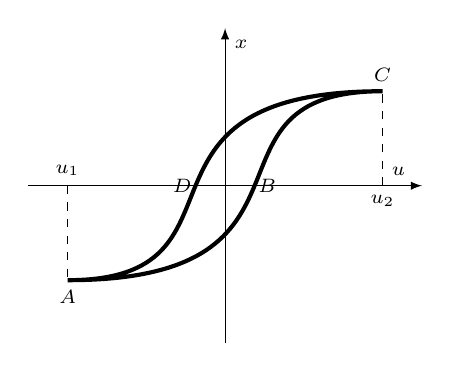
\begin{tikzpicture}
  

    \draw[line width=1.5pt] (-2,-1.2) .. controls (1.5,-1.2) and (-0.5,1.2) .. (2,1.2) .. controls (-1.5,1.2) and (0.5,-1.2) ..(-2,-1.2);
    \draw[-latex] (-2.5,0) -- (2.5,0);
    \node[above] at (2.2, 0) {\scriptsize{$u$}};
    \draw[-latex] (0,-2) -- (0,2);
    \node[right] at (0, 1.8) {\scriptsize{$x$}};

    \draw[dashed] (-2,0) node[above]{\scriptsize $u_1$} -- (-2,-1.2)node[below] {\scriptsize $A$};
    \node[right] at (0.3, 0) {\scriptsize $B$};
    \draw[dashed] (2,0) node[below]{\scriptsize $u_2$} -- (2,1.2)node[above] {\scriptsize{$C$}};
    \node[left] at (-0.3, 0) {\scriptsize{$D$}};

\end{tikzpicture}
\end{document}
